Active prosthetic hands, driven by a motor to open and close the ``claw,'' have been around for many years.
Recently, however, advances in mechatronics have improved such hands and currently
various prosthetic hands with 3 or more active degrees of freedom are being put
on the market.  Such hand developments are a result of various robotic hands which are highly humanoid,
light and gifted with a number of degrees of freedom. Attempts in this
sense include, e.g., the DLR prosthetic hand (\cite{Hua2006}---see
Figure \ref{fig:DLRHandII}), the CyberHand project \cite{cyberhand},
and the i-LIMB hand by Touch Bionics \cite{ilimb}.

\begin{figure}
  \begin{tabular}{cc}
    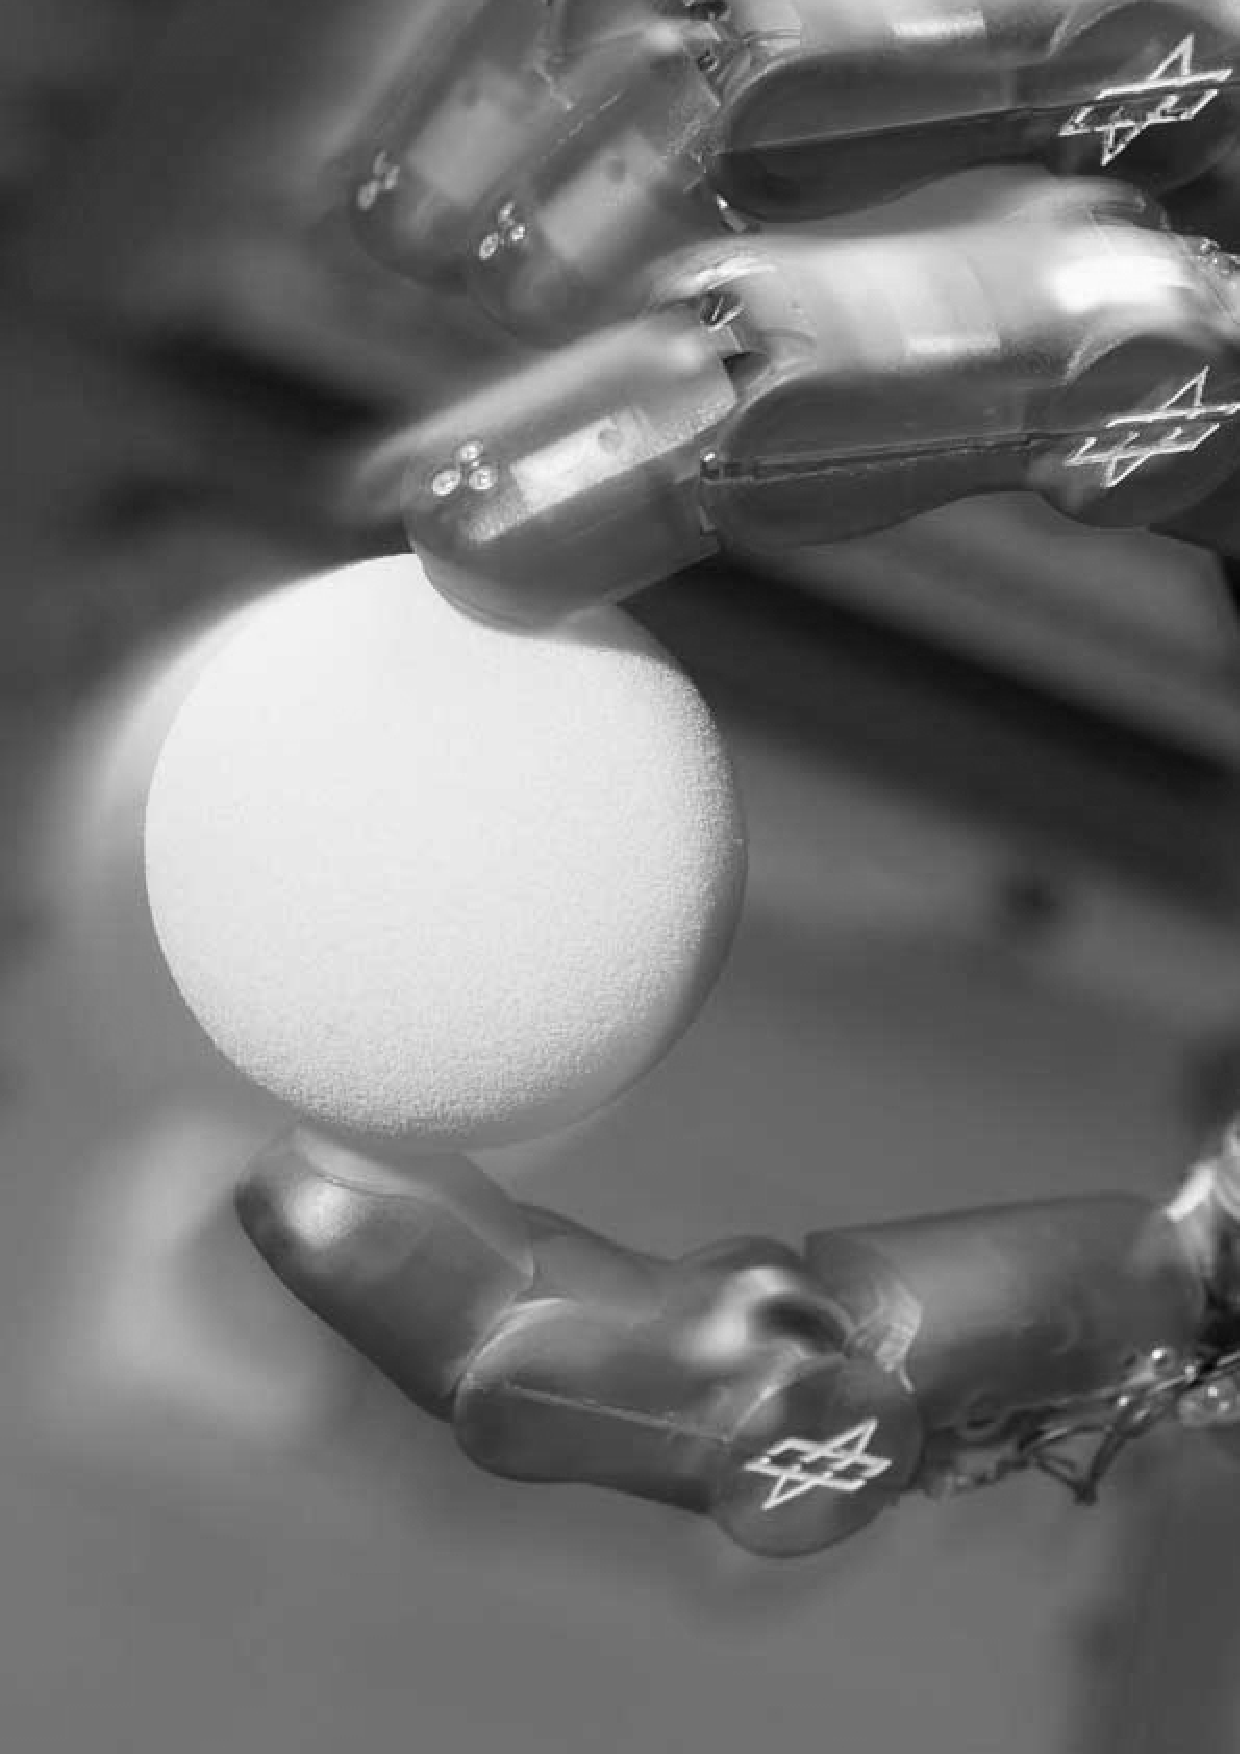
\includegraphics[height=0.12\textheight]{figs/DLRHand-Ball-comp.pdf} &
    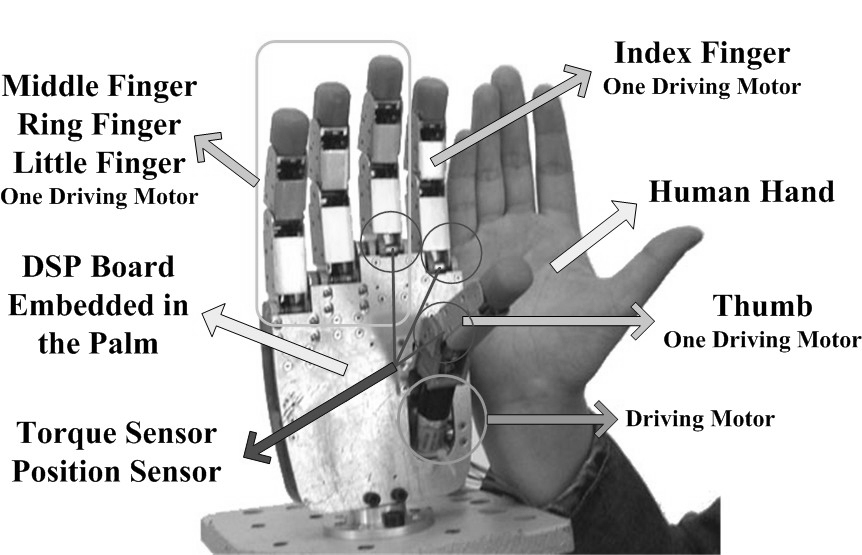
\includegraphics[height=0.12\textheight]{figs/DLR-Prothese.pdf}
  \end{tabular}
  \caption{(left) The DLR Hand II. (right) The DLR prosthetic hand.}
  \label{fig:DLRHandII}
\end{figure}

Still, a general sense of frustration impends, as far as
\emph{control} of the prosthesis is concerned. As a matter of fact,
given the current state of the art, it is basically impossible for the
patient to precisely command the prosthesis what to do; whereas,
operating a hand requires a fine control down to the level of the
single fingers. First of all, presented with a certain task such as
turning a door handle or grabbing a car key, the patient must be able
to enforce the correct grasping type; this involves the activation of
some joints only, and in particular positions. Secondly, the amount of
force involved in the grasp must be controlled, so that it is possible
to grab, e.g., both a hammer without letting it slip and an egg
without breaking it.

To this end, two types of interfaces between the patient and the
prosthesis have been developed or are being studied: \emph{invasive}
and \emph{non-invasive}. The former gather control signals directly
from the user's nervous system, either via brain implants or surgical
use of electrodes. Quite obviously, invasive interfaces are supposed
to deliver a high signal quality, since the signals can be gathered
exactly in the right spots; but they involve surgery and all related
sterility (and psychological) issues. On the other hand, non-invasive
interfaces are easier to handle, manufacture and implant, but require
a much better signal conditioning, since they usually work with
surface (skin) signals or vision and gaze tracking.

In the context of non-invasive interfaces for controlling mechanical
hands, a concrete possibility arises from \emph{forearm surface
electromyography} (EMG), a technique by which muscle
activation potentials are gathered by electrodes placed on the
patient's forearm skin; these potentials can be used to track which
muscles the patient is willing to activate, and with what force.
Surface EMG is therefore, in principle, a cheap and easy way of
detecting what the patient wants the prosthesis to do.

Still, the EMG signal suffers from a number of problems, among which
the unprecise placement of the electrodes, signal drifting and change
due to sweat formation and muscular fatigue and cross-talking among
deep and superficial muscles. It seems, though, that good results can
be obtained via \emph{machine learning} techniques, as shown in, e.g.,
\cite{smagt}. In machine learning, one tries to approximate an unknown
function given its values in a number of samples; the application to
the current problem is exactly that of building a map relating EMG
activation potentials and muscle force, and therefore hand finger
movements.

Such a system must be highly adaptive, accurate and fast---possibly,
able to run in real time, as the patient is wearing the prosthesis.
Another very desirable characteristic is that the system should learn
automatically as the patient moves, being able to understand when new
portions of the input space are being explored, i.e., what new
movements are required of the prosthesis. But so far machine learning
applied to surface EMG has only been able to classify hand postures.
For example, the surface EMG signal can be used to detect whether the
patient is attempting a cylindric grasp or a two-finger grip
\cite{ekvall}; but no indication about the amount of force involved in
the grasping act is detected.

In this paper we show a rather detailed analysis of what machine
learning can do when applied to such a problem. Over several days, we have
gathered forearm surface EMG data while an able-bodied human subject
was gripping in four distinct ways a force sensor; we have then
trained three different machine learning systems to guess, from the
EMG signal,
\begin{enumerate}

  \item what kind of grasp the subject was doing, e.g., thumb and
    index finger, thumb and middle finger, thumb and ring finger or
    thumb and all other fingers; and

  \item how much force the subject was exerting, in order to
    understand whether the grasp was, e.g., a power grasp or rather a
    precision grip. Surprisingly, as far as we know, nobody has ever
    attempted so far to solve this problem, although it is well-known
    that the EMG is related to the force a muscle is exerting.

\end{enumerate}

The three approaches we have experimented with are:
(a) a simple feed-forward neural network with one hidden layer,
(b) a Support Vector Machine with radial basis function kernel
\cite{BGV92}, and (c) Locally Weighted Projection Regression
\cite{lwpr}. Our analysis consists of a preliminary phase in which
several models have been built in a batch fashion, in order to
understand how to deal with the non-stationarity of EMG. The most
interesting challenge has been how to filter out unwanted data, at the
same time keeping a high overall accuracy, both in classification and
regression. Later on, based upon the results obtained in the
preliminary phase, we have developed a simple but effective procedure
for selecting a subset of the samples on-the-fly, called \emph{Online
Uniformisation} (OU).

OU is based upon the simple idea of keeping a minimum inter-sample
Euclidean distance, in order to uniformly sample the input space. The
selected samples are then used to periodically re-train the system,
and check that it has adapted to the new data. The training sets thus
obtained are remarkably small and thus usable on-line, and they offer
an excellent trade-off between size and accuracy. In particular, as a
certain parameter is increased, the size of the uniform training sets
decreases polynomially, while the error rate increases only
linearly; therefore one can obtain much smaller training sets (which
means faster or more adaptive machines) by accepting an error rate
which is only linearly worse.

This behaviour appears in both problems highlighted above (the former
involving classification, the latter regression), and for all the
approaches tested. Our numerical results indicate that, in such a
scenario, the type of grasp can be reconstructed with an average
accuracy of $89.67\% \pm 1.53\%$, and the applied force can be
predicted with an average percentage error of $7.89\% \pm 0.09\%$,
meaning $4.5$N over a range of about $57$N.

The paper is structured as follows: after a brief review of relevant
literature, we describe in detail the experiment and the methods used
to tackle it (Section \ref{sec:m&ms}); then we show and comment on the
experimental results, both the preliminary phase and the online
experiments (Section \ref{sec:exp}); lastly, discussion and
conclusions are presented.
